\subsection{GUI}

\begin{figure}[h]
	\centering
		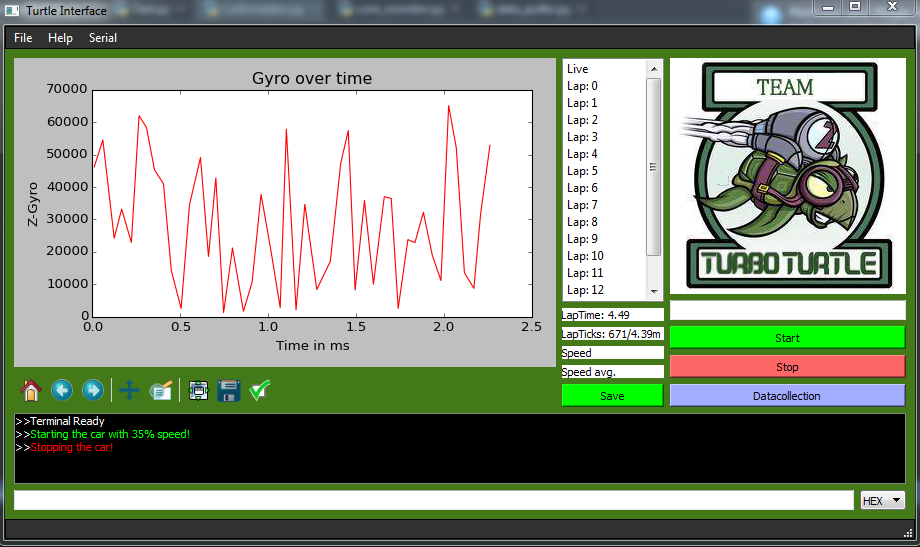
\includegraphics[scale=0.60]{Billeder/Application.PNG}
	\caption{Her ses det GUI vi har fremstillet i Python til at styre bilen og lave dataopsamling. Der er mulighed for at 				starte og stoppe bilen samt indsamle komplete dataset der kan gemmmes. Programmet kan beregne gennemsnitshastighed 				samt øjeblikshastighed af bilen. Der er også en terminal med indbygget farvekodning for kendte kommandoer}
	\label{fig:Application}
\end{figure}

I forbindelse med udviklingen af bilen har vi også udviklet et GUI. Dette har givet os mulighed for at monitorere bilen i real-time. Ved opstart kommer der en dialog der giver mulighed for at vælge com-port og oprette forbindelse til bilen. Derefter kan bilen startes enten via knapper eller via terminal direkte med kommandoer. Når dataopsamling er slået til vil grafen liveopdaterer med de data vi har sat den til at vise. Og for hver gang bilen passere målstregen vil data blive gemt i datasæt som man kan vælge at kigge på senere. Her er der mulighed for at zoome ind og gemme data hvis man har lyst. Selve GUI'et viser altid den nyeste laptid og beregnet gennemsnitshastighed for den lap, samt viser bilens øjeblikshastighed.

